\chapter{ROC curves}
This chapter is based on Ref.\cite{wiki-roc}.

ROC stands for
{\bf  Receiver Operating Characteristic}.
ROC curves are used in binary
classification (BC).

To do BC, we are given the value
$x\in\RR$
for an individual. From this, 
we want to decide
whether that
individual 
has $a=0$
or $a=1$.
The decision will
depend on the
value
of a
{\bf threshold parameter $\tau\in \RR$}.


\begin{figure}[h!]
$$\xymatrix{
\rvx&\rva\ar[l]
}$$
\caption{bnet for 
BC.}
\label{fig-roc-bnet}
\end{figure}
Fig.\ref{fig-roc-bnet}
shows the bnet used for BC.


\begin{figure}[h!]
\centering
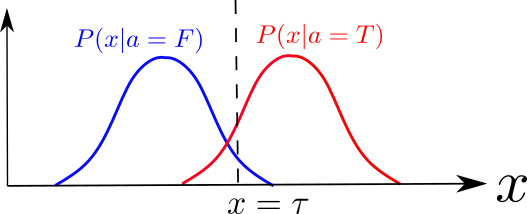
\includegraphics[width=3in]
{roc/bell-curves.png}
\caption{$x$-distribution for
two hypotheses $a=0,1$. } 
\label{fig-bell-curves}
\end{figure}
Fig.\ref{fig-bell-curves}
is a 
plot
of $P(x|a)$, i.e., the TPM 
for node $\rvx$
of the bnet in Fig.\ref{fig-roc-bnet}.


\begin{figure}[h!]
\centering
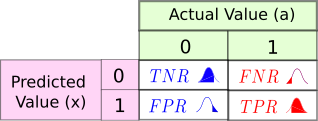
\includegraphics[width=3in]
{roc/confusion-mat.png}
\caption{The confusion matrix 
$P(b|a)$
for BC.} 
\label{fig-confusion-mat}
\end{figure}

Whereas $a$
is binary, $x$
is continuous. 
But we can replace
$x$ by a binary variable

\beq
b=\indi(x>\tau)
\;.
\eeq
$P(b|a)$
for $b, a\in\bool$
is called the
{\bf confusion matrix}
or {\bf contingency table}
for BC.
The confusion
matrix can be
calculated from
the TPM $P(x|a)$.
Fig.\ref{fig-confusion-mat}
illustrates the
confusion matrix
$P(b|a)$
for BC.
In that
figure,
the rates $R$
are defined as
follows.\footnote{
I find the notation 
$x|a$ where $x,a\in \bool$
much clearer than $\alp\beta$
where $\alp=T,F$ and 
$\beta=N,P$.
Note that $\alp=\indi(x=a)$
and $\beta=x$,
if we identify $0=F=N$
and $1=T=P$.}

\begin{itemize}


\item{\color{blue}\bf True Negative Rate (TNR)}
\beqa
\color{blue}
R_{0|0}(\tau)
&=&
 P(x<\tau|a=0)= \int_{x<\tau}dx\;P(x|a=0)
\eeqa

\item {\color{blue}\bf False Positive Rate (FPR)}
\beqa
\color{blue}
R_{1|0}(\tau)&=&
1-R_{0|0}(\tau)
\\
&=&
P(x>\tau|a=0)= \int_{x>\tau}dx\;P(x|a=0)
\eeqa
In Hypothesis Testing,
$R_{1|0}$ is called the {\bf p-value that $\rvx>\tau$
assuming curve $0$ is the
null hypothesis}.

\item {\color{red}\bf False Negative Rate (FNR)}
\beqa
\color{red}
R_{0|1}(\tau)
&=& P(x<\tau|a=1)= \int_{x<\tau}dx\;P(x|a=1)
\eeqa
In Hypothesis Testing,
$R_{0|1}$ is called the 
{\bf p-value that $\rvx<\tau$
assuming curve $1$ is the
null hypothesis}.

\item{\color{red}\bf True Positive  Rate (TPR)}
\beqa
\color{red}
R_{1|1}(\tau)&=& 
1-R_{0|1}(\tau)
\\
&=&
P(x>\tau|a=1)=\int_{x>\tau}dx\;P(x|a=1)
\eeqa


\end{itemize}

\begin{figure}[h!]
\centering
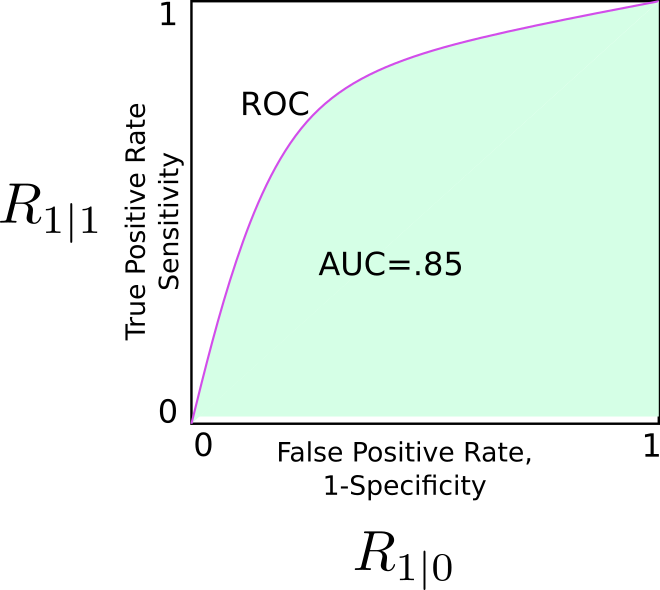
\includegraphics[width=2in]
{roc/roc-auc.png}
\caption{Example of ROC.
Green shaded
 area is the AUC of the ROC.} 
\label{fig-roc-auc}
\end{figure}

\begin{figure}[h!]
\centering
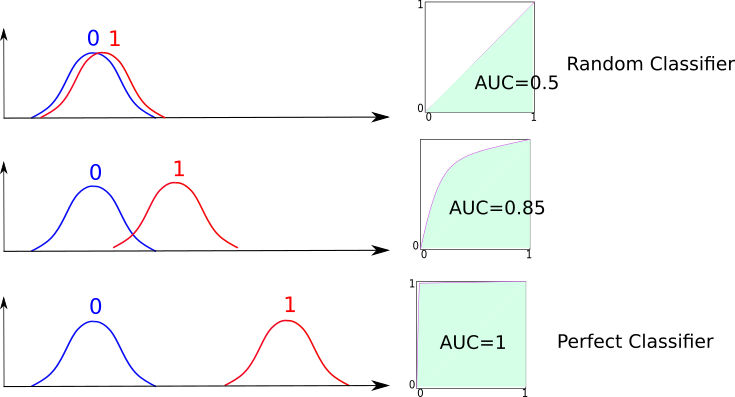
\includegraphics[width=4in]
{roc/roc-panels.png}
\caption{
ROC curves for
3 different separations
between the 0 and 1 
x-distributions.} 
\label{fig-roc-panels}
\end{figure}



The {\bf Receiver Operating Characteristic 
(ROC)} is a
parametric plot with  $X=R_{1|0}(\tau)$
and $Y=R_{1|1}(\tau)$,
where $\tau\in\RR$.
The {\bf Area Under the Curve (AUC)}
is the area under the ROC.
Fig.\ref{fig-roc-auc}
shows an example of a ROC and its AUC.

Fig.\ref{fig-roc-panels} shows
situations that give
AUC=.5 (random classifier),
AUC=.85, and AUC=1 (perfect classifier).
It's also possible to get an $AUC\in[0,0.5]$,
but we will
ignore those models
because they are useless for BC.



Note that

\beqa
AUC &=&\int_{x=0}^1 d\tau\;\;
R_{1|1}(\tau)
\frac{dR_{1|0}(\tau)}{d\tau}
\\
&=&
\int_{\infty}^{{\color{red}-\infty}} d\tau\;\;
\left\{\int_{{\color{red}-\infty}}^\infty dx\;\;
\indi(x>\tau) P(x|a=1)\right\}
(-1)P(x=\tau|a=0)
\\
&=&
\int_{{\color{red}-\infty}}^\infty dx'\;\;
\int_{{\color{red}-\infty}}^\infty dx\;\;
\indi(x>x') P(x|a=1)
P(x'|a=0)
\;.
\eeqa

See Fig.\ref{fig-pregnant-not-pregnant}
for an example of False Positive and False Negative
predictions.

\begin{figure}[h!]
\centering
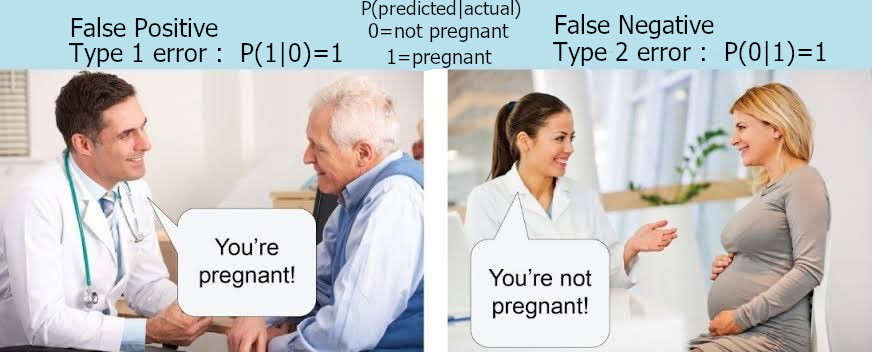
\includegraphics[width=6in]
{roc/pregnant-not-pregnant.jpg}
\caption{Example of False Positive and False Negative predictions.}
\label{fig-pregnant-not-pregnant}
\end{figure}


\section{Terminology Table
Adapted from Wikipedia Ref.\cite{wiki-roc}}

Let 
$N_{x|a}$ be numbers (counts) so that
\beq
P(x|a)=
\frac{ N_{x|a}}
{\sum_{x'} N_{x'|a}}
\eeq
for all $x,a\in \bool$.



condition positive (P):
$N_{|1}=\sum_x N_{x|1}$,
the number of real positive cases in the data

condition negative (N):
$N_{|0}=\sum_x N_{x|0}$,
the number of real negative cases in the data

true positive (TP):
$N_{1|1}$, hit

true negative (TN):
$N_{0|0}$, correct rejection

false positive (FP):
$N_{1|0}$, false alarm, type I error or underestimation

false negative (FN):
$N_{0|1}$, miss, type II error or overestimation

sensitivity, recall, hit rate, or true positive rate 
(TPR):
\beq TPR=
{  {R_{1|1}} ={\frac { {N_{1|1}} }{ {N_{|1}} }}=
{\frac { {N_{1|1}} }{ {N_{1|1}} + {N_{0|1}} }}=1- {R_{0|1}} }
\eeq

specificity, selectivity or true negative rate (TNR):
\beq TNR=
{  {R_{0|0}} ={\frac { {N_{0|0}} }{ {N_{|0}} }}
={\frac { {N_{0|0}} }{ {N_{0|0}} + {N_{1|0}} }}=
1- {R_{1|0}} }
\eeq

precision or positive predictive value (PPV):
\beq 
{  {PPV} ={\frac { {N_{1|1}} }
{ {N_{1|1}} + {N_{1|0}} }}=1- {FDR} }
\eeq

negative predictive value (NPV):
\beq 
{  {NPV} ={\frac { {N_{0|0}} }
{ {N_{0|0}} + {N_{0|1}} }}=1- {FOR} }
\eeq

miss rate or false negative rate (FNR):
\beq FNR=
{  {R_{0|1}} ={\frac { {N_{0|1}} }
{ {N_{|1}} }}={\frac { {N_{0|1}} }{ {N_{0|1}} 
+ {N_{1|1}} }}=1- {R_{1|1}} }
\eeq

fall-out or false positive rate (FPR):
\beq FPR=
{  {R_{1|0}} ={\frac { {N_{1|0}} }
{ {N_{|0}} }}={\frac { {N_{1|0}} }
{ {N_{1|0}} + {N_{0|0}} }}=1- {R_{0|0}} }
\eeq

false discovery rate (FDR):
\beq 
{  {FDR} ={\frac { {N_{1|0}} }
{ {N_{1|0}} + {N_{1|1}} }}=1- {PPV} }
\eeq

false omission rate (FOR):
\beq 
{  {FOR} ={\frac { {N_{0|1}} }
{ {N_{0|1}} + {N_{0|0}} }}=1- {NPV} }
\eeq


accuracy (ACC):
\beq 
{  {ACC} ={\frac { {N_{1|1}} + {N_{0|0}} }
{ {N_{|1}} + {N_{|0}} }}={\frac { {N_{1|1}} + {N_{0|0}} }
{ {N_{1|1}} + {N_{0|0}} + {N_{1|0}} + {N_{0|1}}
 }}}
\eeq

balanced accuracy (BA):
\beq 
{  {BA} ={\frac {R_{1|1}+R_{0|0}}{2}}}
\eeq

F1 score
is the harmonic mean of precision and sensitivity: 
\beq 
{  {F}_{1}=2\times {\frac { {PPV} 
\times  {R_{1|1}} }{ {PPV} + {R_{1|1}} }}=
{\frac {2 {N_{1|1}} }{2 {N_{1|1}} + {N_{1|0}} +
 {N_{0|1}} }}}
\eeq

